% Created with jtex v.1.0.4
\documentclass{article}
\usepackage{arxiv}

\usepackage[utf8]{inputenc} % allow utf-8 input
\usepackage[T1]{fontenc}    % use 8-bit T1 fonts
\usepackage{hyperref}       % hyperlinks
\usepackage{url}            % simple URL typesetting
\usepackage{datetime}       % show dates in the title block
\usepackage{booktabs}       % professional-quality tables
\usepackage{amsfonts}       % blackboard math symbols
\usepackage{nicefrac}       % compact symbols for 1/2, etc.
\usepackage{microtype}      % microtypography
\usepackage{graphicx}
\usepackage{natbib}
\usepackage{doi}
\usepackage{xcolor}

%%%%%%%%%%%%%%%%%%%%%%%%%%%%%%%%%%%%%%%%%%%%%%%%%%
%%%%%%%%%%%%%%%%%%%%  imports  %%%%%%%%%%%%%%%%%%%
\usepackage{amsmath}
%%%%%%%%%%%%%%%%%%%%%%%%%%%%%%%%%%%%%%%%%%%%%%%%%%

\hypersetup{colorlinks = true,
linkcolor = purple,
urlcolor  = blue,
citecolor = cyan,
anchorcolor = black}

\title{The attractor states of the functional brain connectome}

\newdate{articleDate}{24}{7}{2023}
\date{\displaydate{articleDate}}

\makeatletter
\let\@fnsymbol\@arabic
\makeatother

\author{Robert Englert\\
University Medicine Essen\\\AND
Tamas Spisak\footnotemark[1]\\
University Medicine Essen\\}

% Uncomment to override  the `A preprint' in the header
\renewcommand{\headeright}{Preprint}
\renewcommand{\undertitle}{}
\renewcommand{\shorttitle}{ConnAttractor Preprint}

%% Add PDF metadata to help others organize their library
%% Once the PDF is generated, you can check the metadata with
%% $ pdfinfo template.pdf
\hypersetup{
pdftitle={\@title},
pdfsubject={},
pdfauthor={\@author},
pdfkeywords={},
addtopdfcreator={Written in Curvenote}
}

\begin{document}
\maketitle
\footnotetext[1]{Correspondence to: tamas.spisak@uk-essen.de}

\begin{abstract}
\textbf{Abstract:}

todo
\end{abstract}

\keywords{}

\textbf{Key Points:}

\begin{itemize}
\item We present a simple yet powerful computational model large-scale brain dynamics
\item The model computes "activity flow" across brain regions using a continuous Hopfield artificial neural network.
\item Instead of training the network weights to solve specific tasks, they are initialized with empirical functional brain
connectivity.
\item It defines an energy level for any arbitrary brain activation patterns and a trajectory towards one of the finite
number of stable patterns (attractor states) that minimize this energy
\item The model captures the dynamic repertoire of the brain in resting conditions
\item It conceptualizes both task-induced and pathological changes in brain activity as a shift in these dynamics.
\item We validate the model through eight studies involving approximately 2000 participants.
\end{itemize}

\section{Introduction}\label{Introduction}

Brain function is characterized by the continuous activation and deactivation of anatomically distributed neuronal
populations.
While the focus of related research is often on the direct mapping between changes in the activity of a single brain
area and a specific task or condition, in reality, regional activation never seems to occur in isolation
\citep{bassett2017network}.

Irrespective of the presence or absence of explicit stimuli, brain regions appear to work in concert, giving rise to a
rich and complex spatiotemporal fluctuation \citep{gutierrez2019infraslow}.
This fluctuation is neither random, nor stationary over time \citep{liu2013time, zalesky2014time}.
It exhibits quasi-periodic properties \citep{thompson2014quasi}, with a limited number of
recurring patterns known as "brain states" \citep{greene2023everyone, vidaurre2017brain, liu2013time, richiardi2011decoding}.

From hidden Markov models, to point-process analyses, a wide variety of descriptive techniques have been previously
employed to characterize whole-brain dynamics. \citep{smith2012temporally, vidaurre2017brain, liu2013time, chen2018human},
providing accumulating evidence not only for the existence of dynamic brain states but also for their clinical
significance. \citep{hutchison2013dynamic, barttfeld2015signature, meer2020movie}.
However, the underlying driving forces remain elusive due to the descriptive nature of such studies.

Brain state dynamics can be assessed with multiple techniques, such as dynamic connectivity analysis (), independent
component analysis \citep{smith2012temporally}, hidden markov models \citep{vidaurre2017brain},
clustering \citep{chen2018human} or point-process analyses to
capture co-activation patterns (CAPs, \citep{liu2013time, chen2015introducing, liu2013decomposition, meer2020movie}.

Questions regarding the mechanisms, that cause these remarkable dynamics, can be addressed through approaches that are
based on computational models, which have the potential to shift our understanding from mere associations to causal
explanations.
Conventional computational approaches attempt to solve this puzzle by going all the way to the biophysical properties
of single neurons, and aim to construct a model of larger neural populations, or even the entire brain
\citep{breakspear2017dynamic}.
Although these approaches have shown numerous successful applications \citep{kriegeskorte2018cognitive, heinz2019towards},
the estimation of all the free parameters in such models presents a grand challenge.
This hampers the ability of these techniques to effectively bridge the gap between explanations at the level of single
neurons and the complexity of behavior \citep{breakspear2017dynamic}.

An alternative approach, known as "neuroconnectomism" \citep{doerig2023neuroconnectionist} shifts the
emphasis from "biophysical fidelity" of models to "cognitive/behavioral fidelity"
\citep{kriegeskorte2018cognitive}, by using artificial neural networks (ANNs) that are trained to
perform various tasks, as brain models.
While this novel paradigm has already made significant contributions to expanding our understanding of the general
computational principles of the brain (see \citep{doerig2023neuroconnectionist}, the need to train ANNs for
specific tasks inherently limits their ability to explain the spontaneous, and largely task-independent, macro-scale
dynamics of neural activity \citep{richards2019deep}.

In this work, we adopt a middle ground between traditional computational modeling and neuroconnectionism to investigate
the phenomenon of brain dynamics.
Similar to neuroconnectionism, our objective is not to attain a comprehensive bottom-up understanding of neural
mechanisms. Therefore, we utilize an artificial neural network (ANN) as a high-level computational model of the
brain (Figure~\ref{concept}A).
However, we do not train our ANN for a specific task, instead we set its weights empirically, with data based
on the "activity flow" \citep{cole2016activity, ito2017cognitive}
across regions within the functional brain connectome, as measured with functional magnetic resonance imaging
(fMRI, Figure~\ref{concept}B).

We employ this neurobiologically motivated ANN architecture, based on the established architecture of a continuous-space
Hopfield network \citep{hopfield1982neural, krotov2023new}.
Within this architecture, the topology of the functional connectome naturally establishes an "energy" level for any
arbitrary activation patterns and determines a trajectory towards one of the finite number of stable patterns, known as
attractor states, that minimize this energy.
In the presence of weak noise, the system does not reach equilibrium (i.e. it does not converge to an attractor state).
Instead, it traverses extensive regions of the state space, with dynamics influenced by multiple attractor states,
arising form the topology of the functional brain connectome (Figure~\ref{concept}C).
Through this walk across the state space, our model also offers a natural explanation for brain state dynamics.

\begin{figure}[!htbp]
\centering
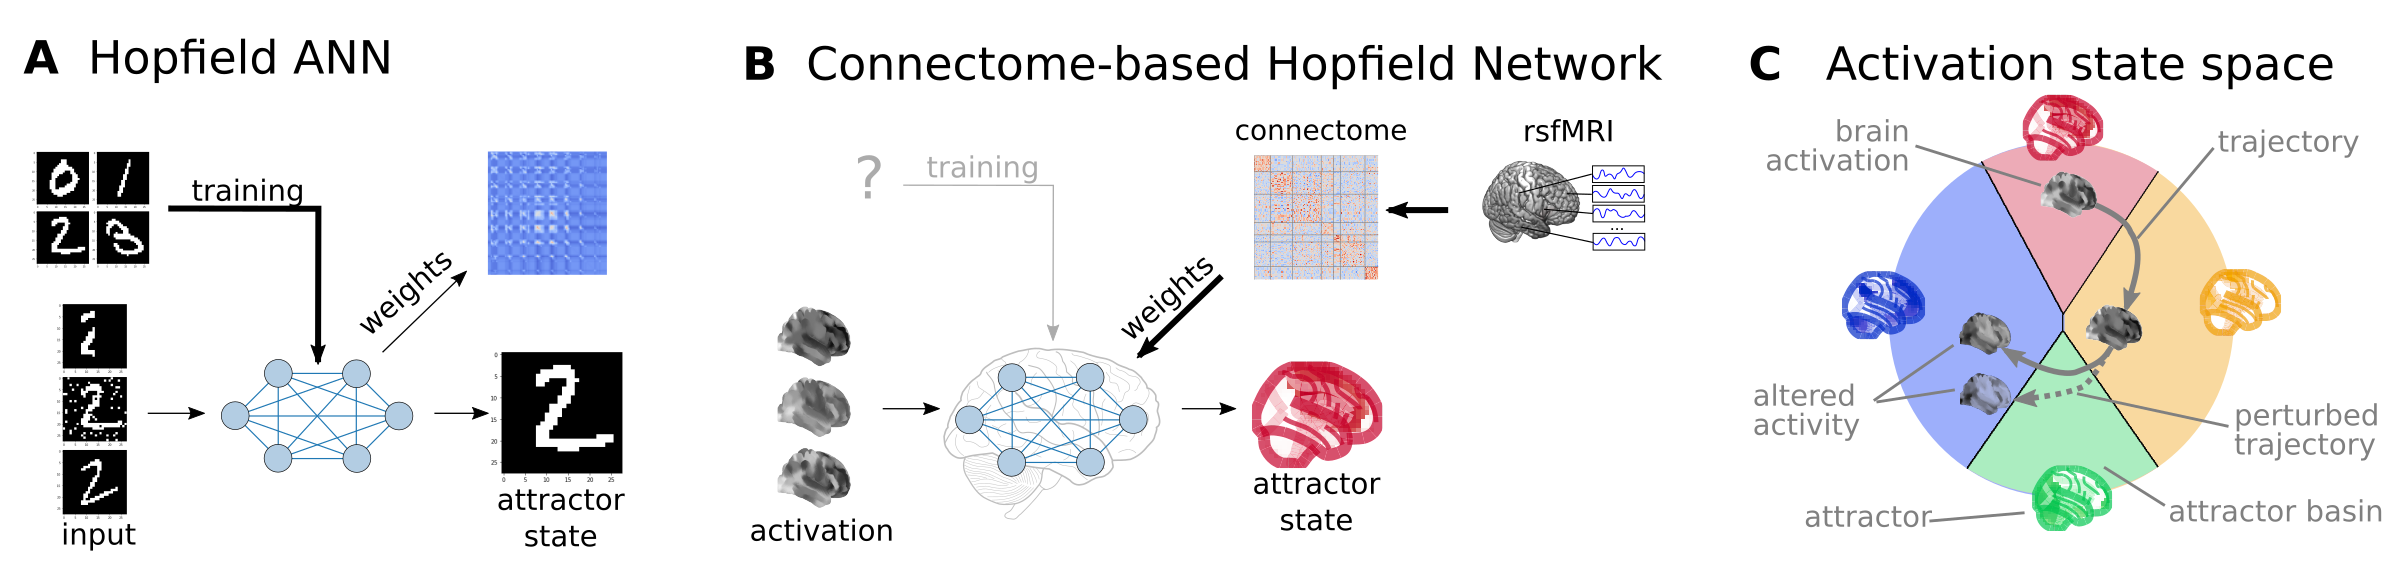
\includegraphics[width=0.7\linewidth]{files/concept-13314c11edf775d931f0384f34726cfb.png}
\caption[]{\textbf{Connectome-based Hopfield networks as models of macro-scale brain dynamics.} \newline
\newline

\textbf{A} Hopfield artificial neural networks (ANNs)  are a form of recurrent ANNs that serve as content-addressable
("associative") memory systems. Hopfield networks can be trained to store a finite number of patterns (e.g. via
Hebbian learning). During the training procedure, the weights of the Hopfield ANN are trained so that the stored
patterns become stable attractor states of the network. Thus, when the trained network is presented partial or noisy
variations of the stored patterns, it can effectively reconstruct the original pattern via an iterative relaxation
procedure that converges to the attractor states.
\textbf{B} We consider regions of the brain as nodes of a Hopfield network. Instead of training the Hopfield network to
specific tasks, we use the set its weights empirically, with the interregional activity flow estimated via functional
brain connectivity. Following form the strong analogies between the relaxation rule of Hopfield networks and the
activity flow principle that links activity to connectivity in brain networks, we propose the constructed
connectome-based Hopfield (CBH) network as a computational model for macro-scale brain dynamics.\newline
\textbf{C} The proposed computational framework assigns an energy level, an attractor state and a position in a
low-dimensional embedding to brain activation patterns. Additionally, it models how the entire state-space of viable
activation patterns is restricted by the dynamics of the system and how alterations in activity and/or connectivity
modify these dynamics.}
\label{concept}
\end{figure}

In this simplistic yet powerful framework, both spontaneous and task-induced brain dynamics can be conceptualized as a
winding, high-dimensional path that meanders on the energy landscape, restricted by the "gravitational pull" of the
attractors states.
The framework provides a generative model for both resting state and task-related brain dynamics, offering novel
perspectives on the mechanistic origins of resting state brain states and task-based activation maps.

In the present work, we first explore the attractor states of the functional brain connectome and construct a
low-dimensional representation of the energy landscape.
Subsequently, we rigorously test the proposed model through a series of experiments, conducted on data obtained
from 8 experimental and clincial studies, encompassing a total of n$\approx$2000 individuals.
These analyses encompass the evaluation of robustness and replicability, testing the model's ability to reconstruct
various characteristics of resting state brain dynamics, as well as its capacity to detect and explain changes induced
by experimental tasks or alterations characteristic to brain disorders.

These experiments provide converging evidence for the validity of connectome-based Hopfield networks (CBH) as models
of brain dynamics, and highlight their potential to provide a fresh perspective on a wide range of research questions
in basic and translational neuroscience.

\section{Results}\label{Results}

\subsection{Connectome-based Hopfield network as a model of brain dynamics}\label{Connectome-based Hopfield network as a model of brain dynamics}

First, we explored the attractor states of the functional brain connectome in a sample of n=41 healthy young
participants (Table~\ref{tab-samples}). We estimated interregional activity flow \citep{cole2016activity, ito2017cognitive}
as the study-level average of regularized partial correlations among the resting state fMRI timeseries of m = 122
functionally defined brain regions (BASC brain atlas, see Methods for details). We then used the standardized
functional connectome as the $w_{ij}$  weights of a continuous-state Hopfield network
\citep{hopfield1982neural, koiran1994dynamics} consisting of $m$ neural units, each having an activity
$a_i \in [ -1,1]$. Hopfield networks can be initialized by an arbitrary activation pattern (consisting of
$m$ activation values) and iteratively updated until convergence is reached (i.e. "relaxed"), according to the
following equation:

\begin{equation}
\label{hopfield-update}
\dot{a}_i = S(\beta \sum_{j=1}^m w_{ij}a_j - b_i)
\end{equation}

where $\dot{a}_i$ is the activity of neural unit $i$ in the next iteration and $S(a_j)$ is the sigmoidal activation
function $S(a) = tanh(a)$ and $b_i$ is the bias of unit $i$ and $\beta$ is the so-called temperature parameter. For
the sake of simplicity, we set $b_i=0$ in all our experiments. We refer to this architecture as a connectome-based
Hopfield network (CBH network). Importantly, the relaxation of a CBH network can be conceptualized as the repeated
application of the activity flow principle \citep{cole2016activity, ito2017cognitive} , simultaneously for all
regions: $\dot{a}_i = \sum_{j=1}^m w_{ij}a_j$. The update rule also exhibits strong analogies with the inner workings
of neural mass models \citep{breakspear2017dynamic} as applied e.g. in dynamic causal modeling(see Discussion for
further details).

Hopfield networks assign an energy value to each possible activity configuration (see Methods), which decreases during
the relaxation procedure until reaching an equilibrium state with minimal energy (Figure~\ref{attractors}A, top panel,
\citep{hopfield1982neural, koiran1994dynamics}.
We used a large number of random initializations to obtain all possible attractor states of the connectome-based
Hopfield network in study 1 (Figure~\ref{attractors}A, bottom panel).

\begin{figure}[!htbp]
\centering
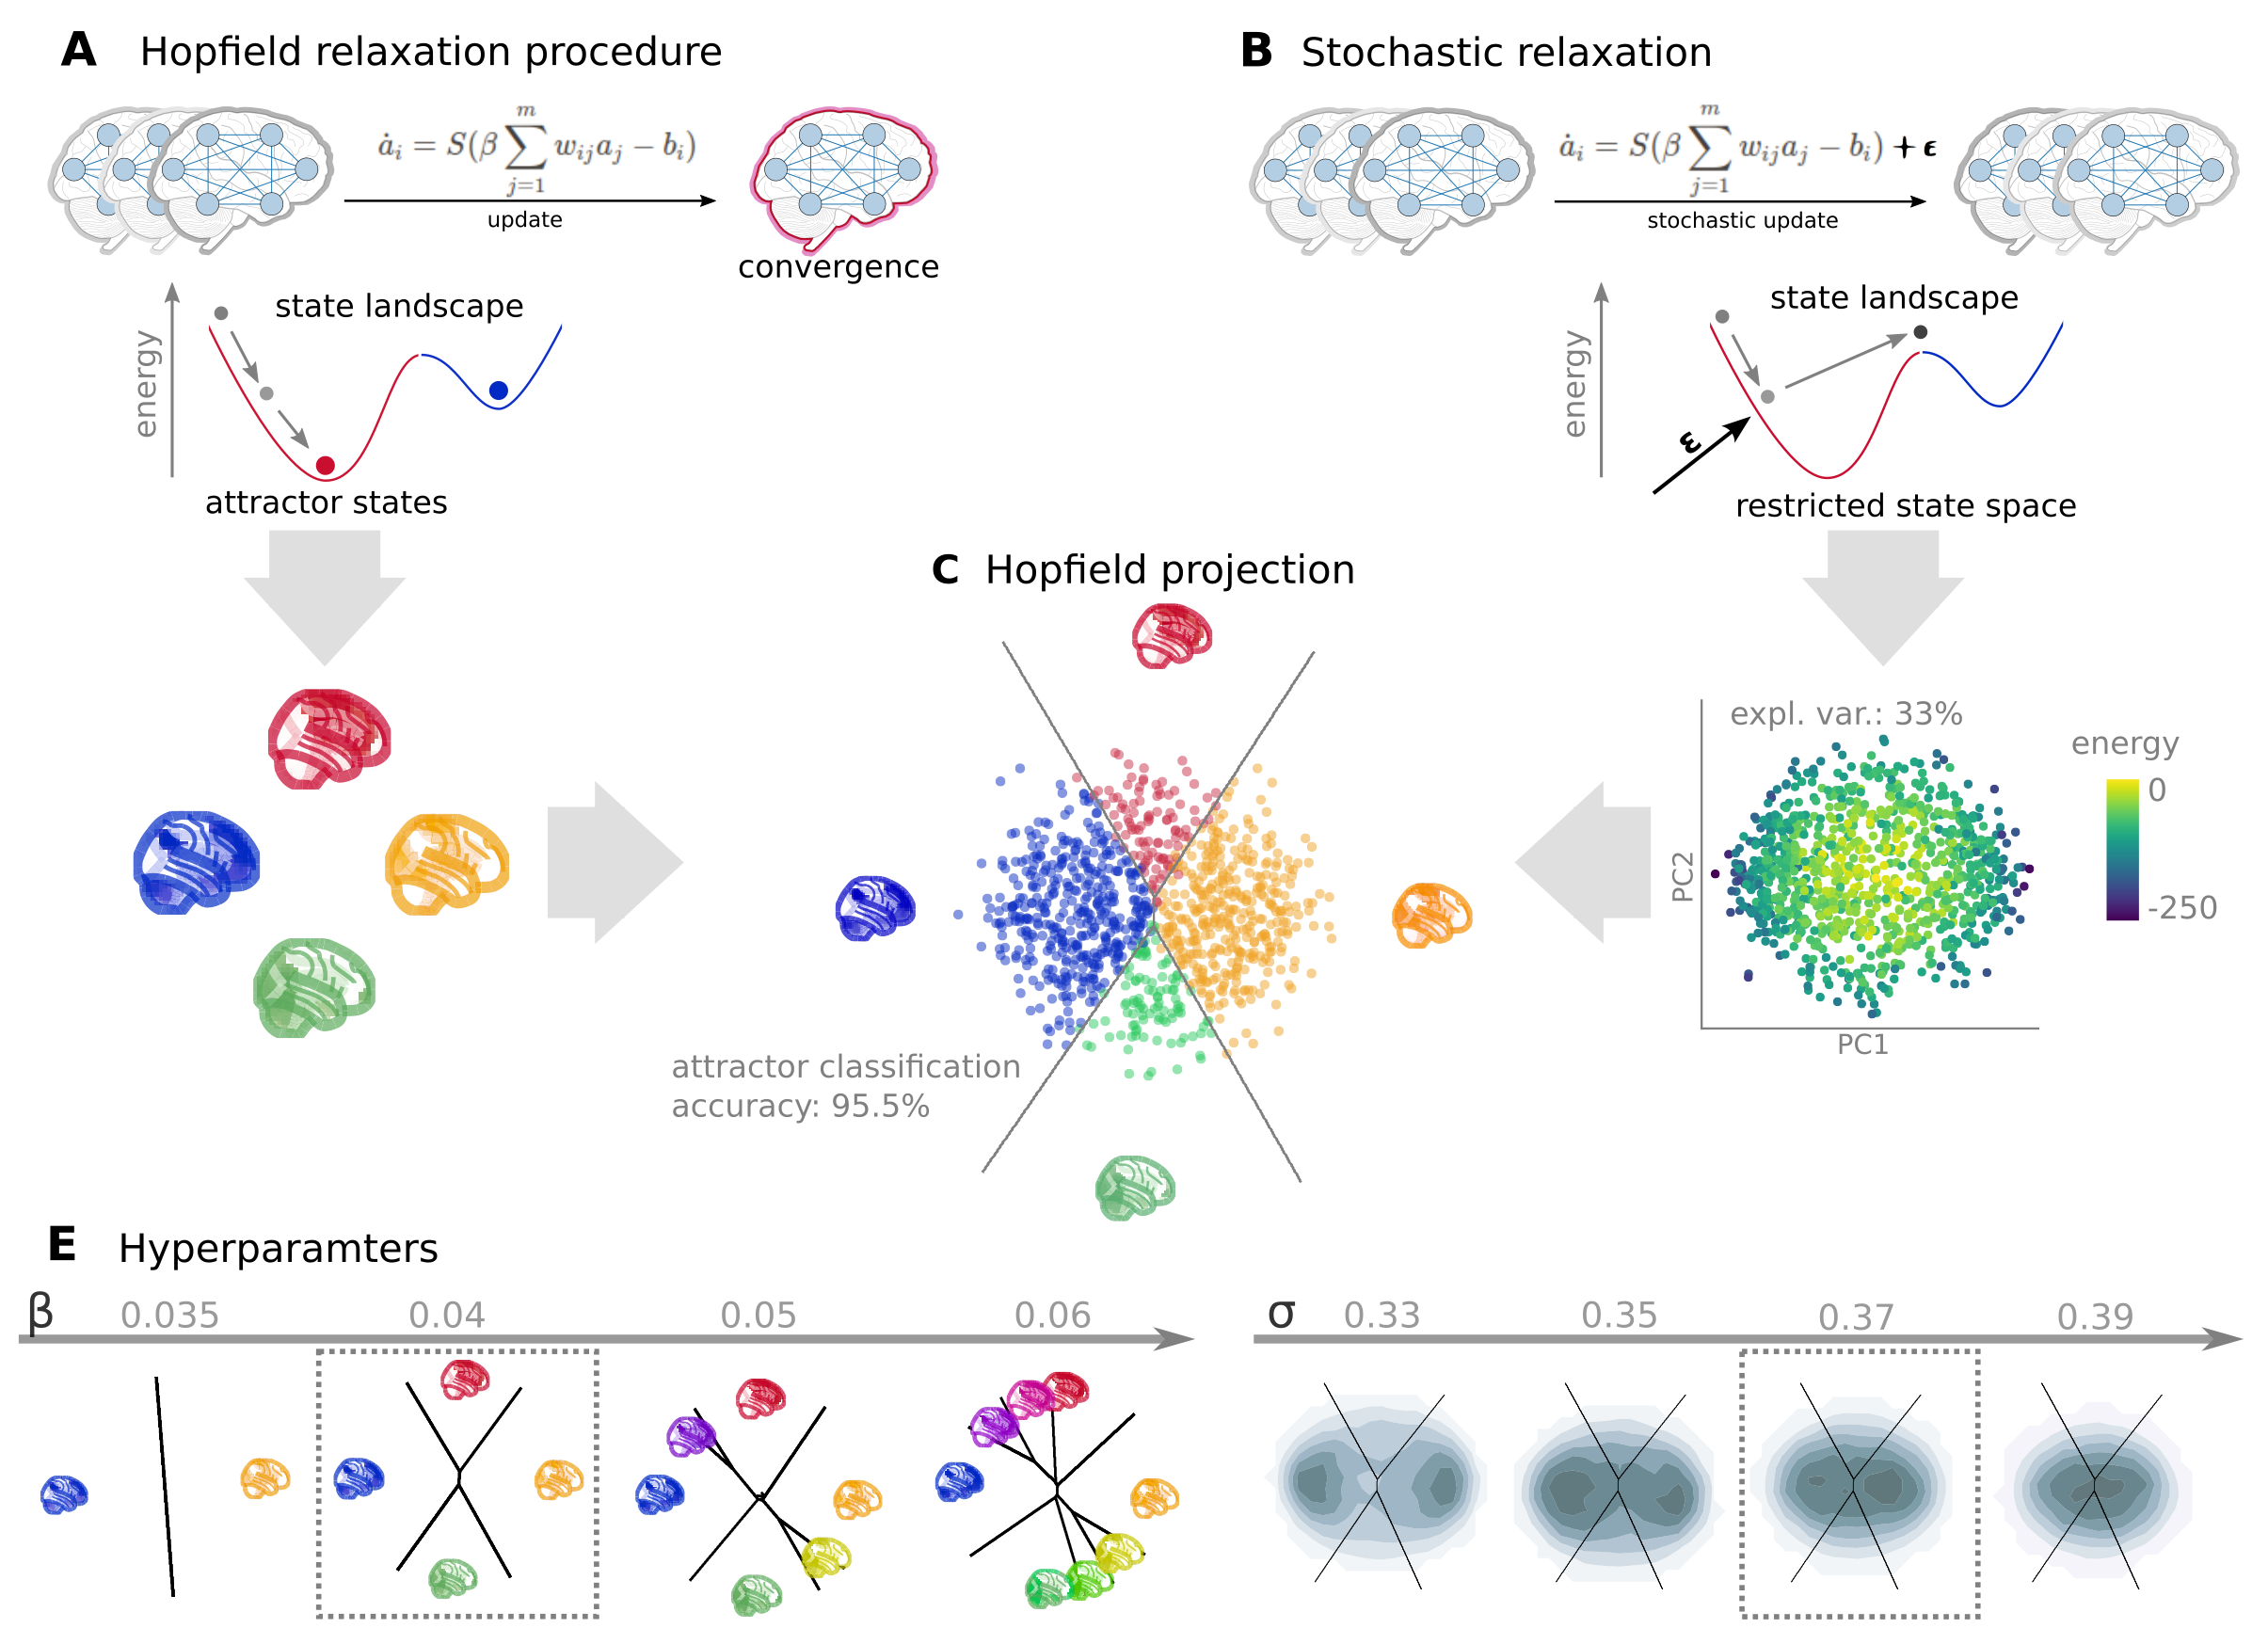
\includegraphics[width=0.7\linewidth]{files/embedding_method-e1585cdac787b467f0ec871e2979ba20.png}
\caption[]{\textbf{Attractor states and state-space dynamics of connectome-based Hopfield networks} \newline
\newline

\textbf{A} Top: During so-called relaxation procedure, activities in the nodes of a connectome-based Hopfield (CBH) network
are iteratively updated based on the activity of all other regions and the connectivity between them. The energy of a
connectome-based Hopfield network decreases during the relaxation procedure until reaching an equilibrium state with
minimal energy, i.e. an attractor state. Bottom: Four attractor states obtained by a CBH, initialized with a
group-level functional connectivity matrix from Table~\ref{tab-samples} (n=44).
\textbf{B} Top: Similarly to stochastic dynamic causal modeling, in presence of weak noise (stochastic update), the system
does not converge to an equilibrium anymore. Instead, it the system transverses on the state landscape in a way
restricted by the topology of the connectome and the "gravitational pull" of the attractor states. Bottom: We sample
the state space by running the stochastic relaxation procedure for an extended amount of time (e.g. 100.000 consecutive
stochatsic updates), each point representing a possible activation configuration (state). To construct a
low-dimensional representation of the state space, we take the first principal components of the simulated activity
patterns. The first two principal components explain approximately 55-85\% of the variance of state energy (depending
on the noise parameter $\sigma$, see Supplementary Material \textbf{X}).
\textbf{C} We map all states of the state space sample to their corresponding attractor state, with the conventional
Hopfield relaxation procedure (A). The four attractor states are also visualized in their corresponding position on the
PCA-based projection. The first two principal components yield a clear separation of the attractive state basins
(cross-validated classification accuracy: 95.5\%, Supplementary Material \textbf{X}). We refer to the resulting visualization
as the Hopfiled projection and use it to visualize CBH-derived and empirical brain dynamics throughout the rest of
the manuscript.
\textbf{E} At its simpliest form, the CBH framework entails only two free hyperparamters: the temperature parameter
$\beta$ (left) that controls the number of attractor states and the noise parameter of the stochastic relaxation
$\sigma$. To avoid overfitting these parameters to the empirical data, we set $\beta=0.4$ and $\sigma=0.01$ for the
rest of the paper.}
\label{attractors}
\end{figure}

Consistent with theoretical expectations, we observed that increasing the temperature parameter $\beta$ led to an
increasing number of attractor states ((Figure~\ref{attractors}E, left), appearing in symmetric pairs
(i.e. $a_i^{(1)} = -a_i^{(2)}$).For simplicity, we set the temperature parameter for the rest of the paper to a value
resulting in 4 distinct attractor states ($\beta=0.4$).

Connectome-based Hopfield networks, without any modifications, always converge to an equilibrium state.
To incorporate stochastic fluctuations in neuronal activity \citep{robinson2005multiscale}, we introduce weak
Gaussian noise to the CBH relaxation procedure. This procedure, referred to as stochastic relaxation, prevents the
system from reaching equilibrium and, somewhat similarly to Stochastic DCM \citep{daunizeau2012stochastic}, induces
complex CBH system dynamics  (equivalent to brain activity fluctuations in our framework) that may traverse extensive
regions of the state space, determined by the "gravity field" (basins) of multiple attractor states (Figure~\ref{attractors}B).

We hypothesise that the resulting dynamics capture essential characteristics of spontaneous activity fluctuations in
the brain and can serve as a valuable generative computational model for large-scale brain dynamics. To sample the
resulting state space, we obtained 100,000 iterations of the stochastic relaxation procedure with a Hopfield network
initialized with the mean functional connectome in study 1. Next, in order to enhance interpretability, we conducted a
principal component analysis (PCA) on the resulting state space sample and obtained the first two principal components.
These components were used to construct a low-dimensional embedding. Largely independent on the free parameter $\sigma$
(variance of the noise), the first two principal components (PCs) explained around 15\% of the variance in the state
space, with attractor states (minimal energy) located at the extremes of the PCs (Figure~\ref{attractors}B, bottom plot).

The PCA embedding exhibited high consistency across different values of $\beta$ and $\sigma$ (Figure~\ref{attractors}E).
For all subsequent analyses, we set $\sigma=0.37$, which was determined through a coarse optimization procedure aimed
at reconstructing the bimodal distribution of empirical data in the same projection (Figure~\ref{attractors}E,
see Methods for details). On the low-dimensional embedding, which we refer to as the \textit{Hopfield projection}, we observed
a clear separation of the attractor states (Figure~\ref{attractors}C), with the two symmetric pairs of attractor states
located at the extremes of the first and second PC. To map the attractor basins on the space spanned by the first two
PCs (Figure~\ref{attractors}C), we obtained the attractor state of each point visited during the stochastic relaxation
and fit a multinomial logistic regression model to predict the attractor state from the first two PCs. The resulting
model demonstrated high prediction accuracy, achieving an out-of-sample accuracy of 96.5\%. The attractor basins were
visualized by using the decision boundaries obtained from this model. (Figure~\ref{attractors}C). We propose the Hopfield
projection depicted on (Figure~\ref{attractors}C) as a simplified representation of brain dynamics, and use it as a basis
for all subsequent analyses in this work.

\subsection{Reconstruction of resting state brain dynamics}\label{Reconstruction of resting state brain dynamics}

The obtained attractor states closely resemble frequently described brain patterns. (\{numref\}rest-validityA). The first
pair of attractors (mapped on PC1) resemble the two complementary ``macro'' systems described by and as well as the two
primary brain states previously described by . This state-pair has previously been described as an ``extrinsic'' system
which exhibits a stronger direct connection to the immediate sensory environment and an "intrinsic" system, whose
activity is primarily associated with dynamic changes in higher-level internal context and closely linked to the default
mode network. The other pair of attractors spans an orthogonal axis connecting regions that are commonly associated
with perception--action cycles

\begin{figure}[!htbp]
\centering
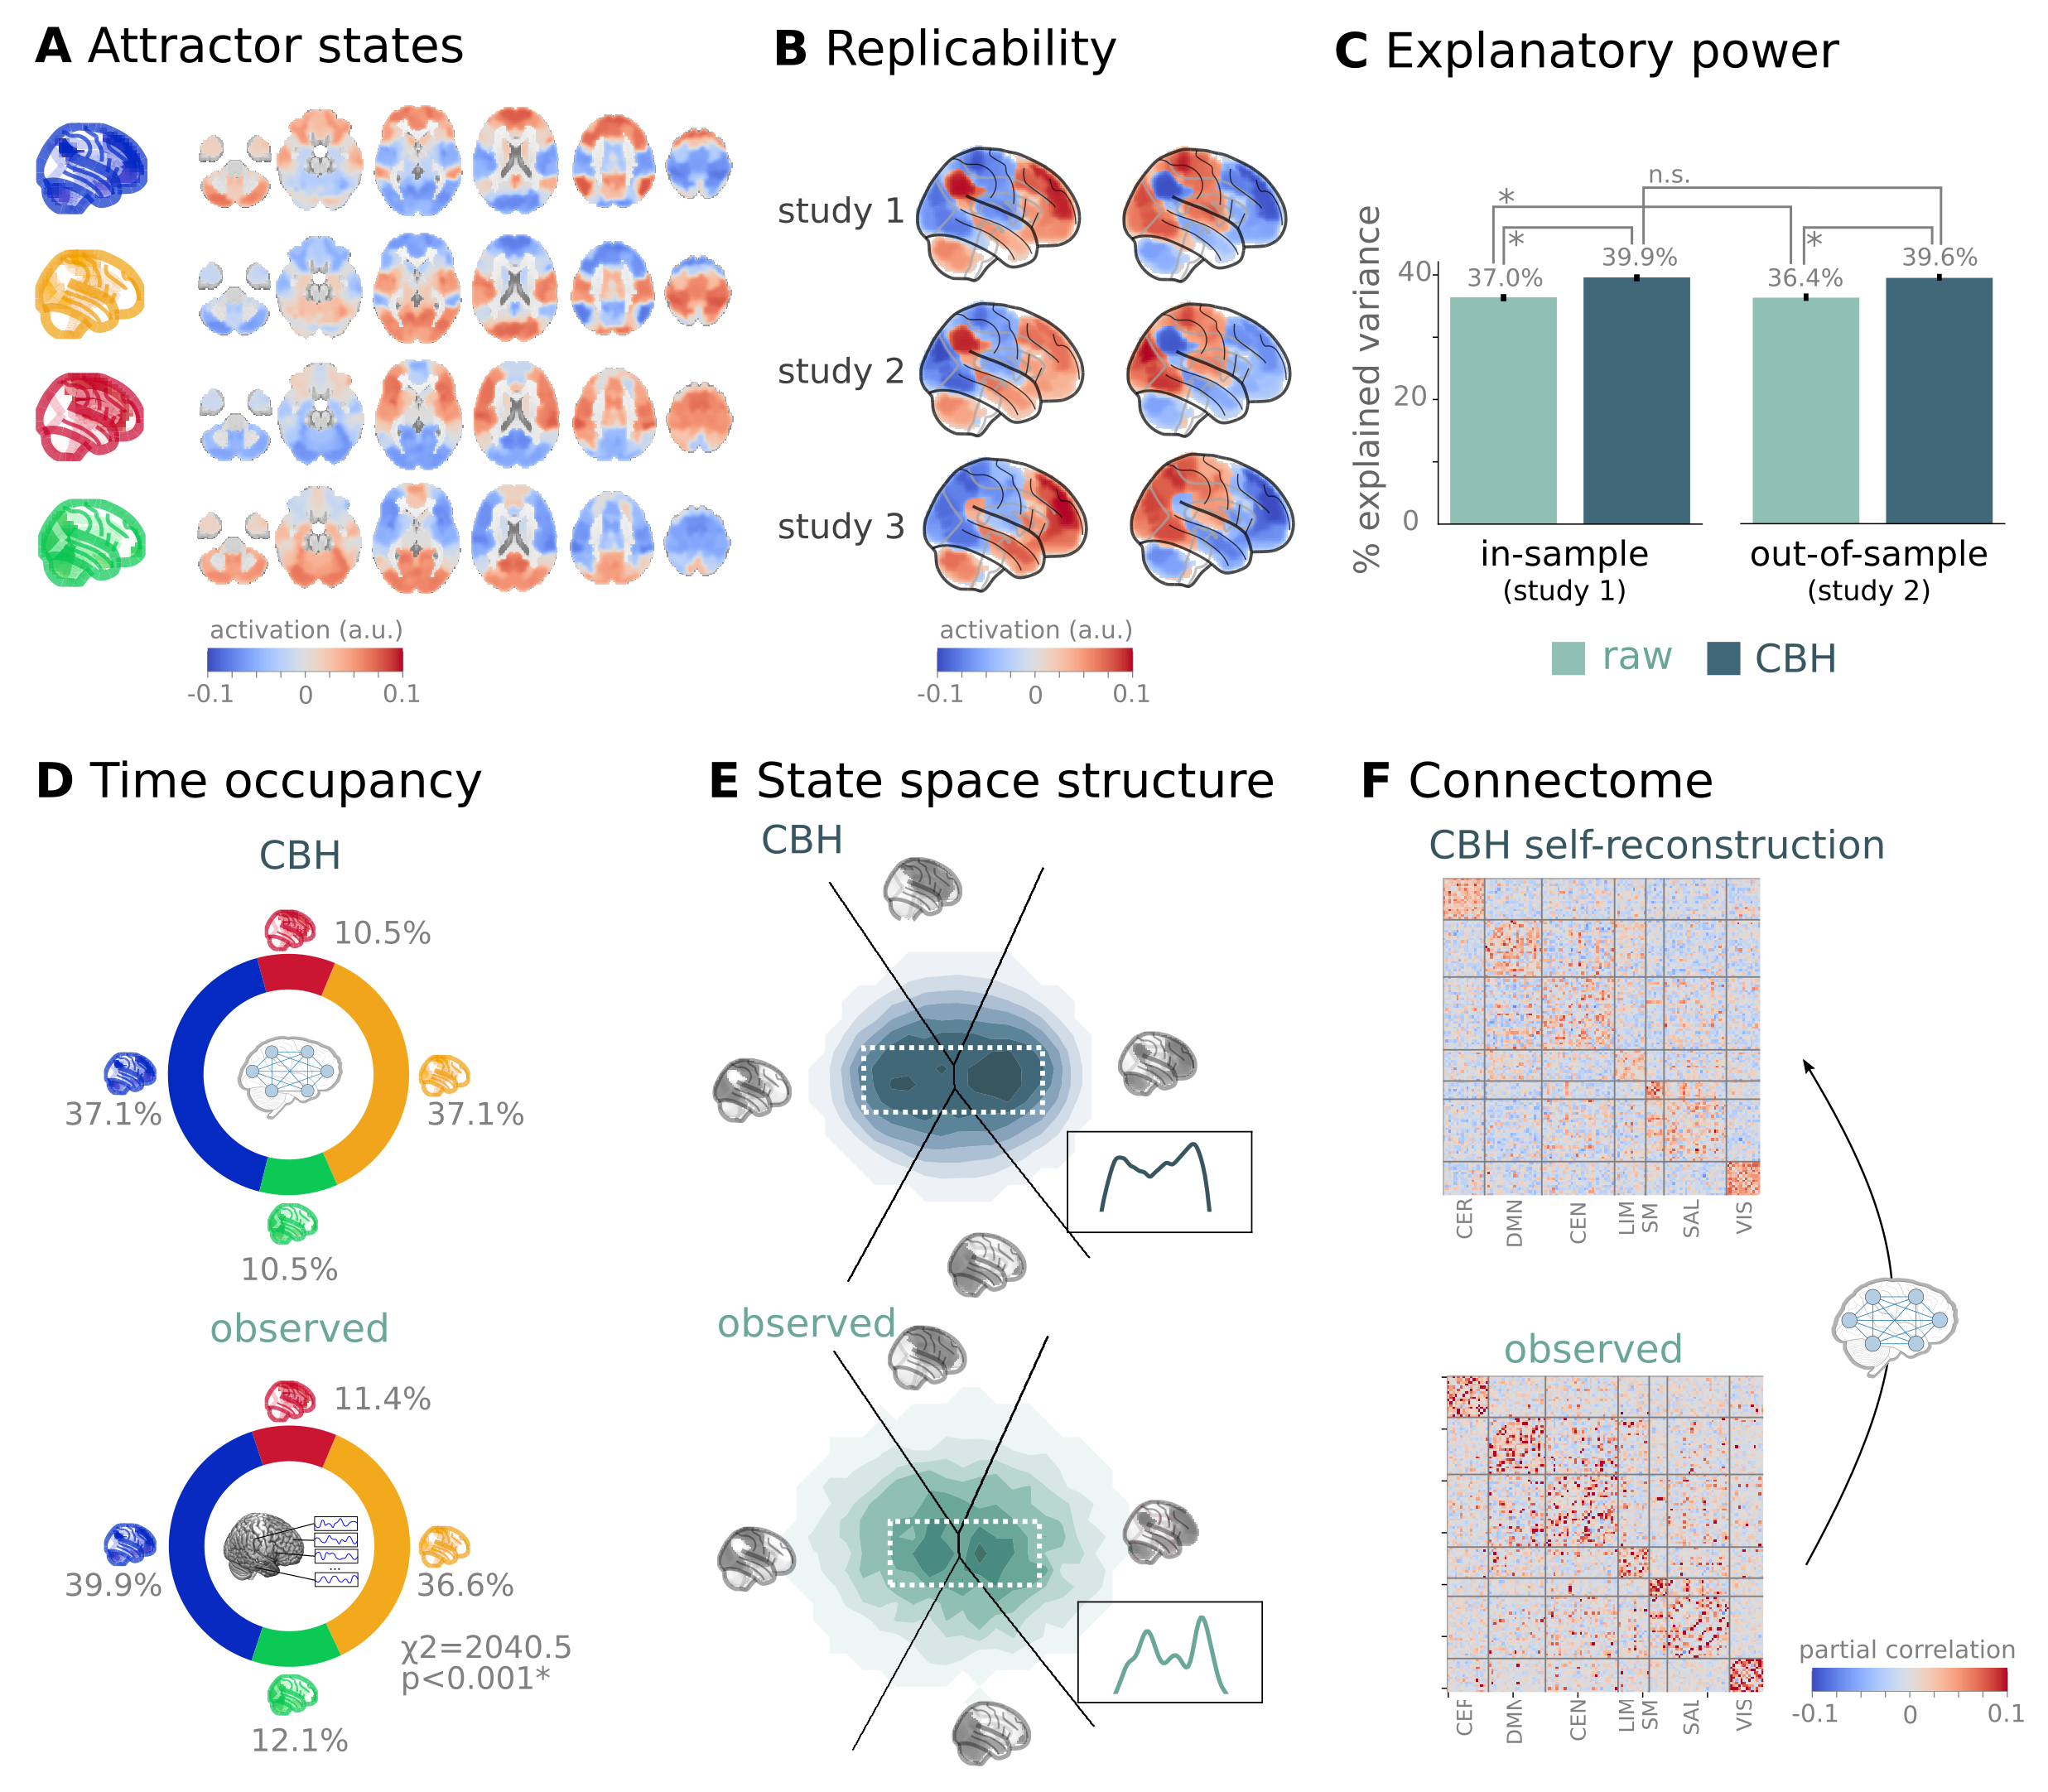
\includegraphics[width=0.7\linewidth]{files/face_validity-f81988c2f14d7470a7ac1b322e6bb29e.png}
\caption[]{\textbf{Connectome-based Hopfield networks reconstruct characteristics of real resting state brain activity.}\newline
\newline

\textbf{A} The four attractor states of the connectome-based Hopfiled (CBH) network from study 1 reflect brain activation
patterns with a high neurobiologicasl relevance, resembling to sub-systems previously described as being associated for
"internal context" (blue), "external context" (yellow), "action/execution" (red) and "perception" (green)\newline
\citep{golland2008data, cioli2014differences, chen2018human, fuster2004upper}.
\textbf{B} The attractor states show excellent replicability in two external datasets (study 2 and 3, mean correlation 0.93).
\textbf{C} The Hopfield projection (first two PCs of the CBH state space) explains more variance (p\textless 0.0001) in the real
resting state fMRI data than principal components derived from the real resting state data itself and generalizes
better (p\textless 0.0001) to out-of-sample data (study 2). Error bars denote 99\% bootstrapped confidence intervals.
\textbf{D} The CBH analysis accurately predicts (p\textless 0.0001) the fraction of time spent on the basis of the four attractor
states in real restring state fMRI data (study 1) and
\textbf{E} reconstructs the characteristic bimodal distribution of the real resting state data.
\textbf{F} CBH networks perform self-reconstruction: the timeseries resulting from the stochastic relaxation procedure
mirror the co-variance structure of the functional connectome the CBH network was initialized with.}
\label{rest-validity}
\end{figure}

Importantly, the discovered attractor states demonstrate a remarkable level of replicability (mean Pearson's
correlation 0.93) across the discovery datasets (study 1) and two independent replication datasets
(Table~\ref{tab-samples}, Figure~\ref{rest-validity}C). This is in line with the previously described, high
robustness of Hopfield networks to noisy input \citep{hopfield1982neural} as well as their ability to tolerate
corrupted weights. (\textbf{ref}, Supplementary Material \textbf{X}) and renders CBH networks highly promising for computational
analyses of brain dynamics.

Further analysis in study 1 showed that connectome-based Hopfield models accurately reconstructed multiple
characteristics of true resting-state data. First, the Hopfield projection accounted for a substantial amount of
variance in the real resting-state fMRI data in study 1 (mean $R^2=0.15$) and generalized well to study 2
(mean $R^2=0.13$) and study 3 (mean $R^2=0.12$) (Figure~\ref{rest-validity}E). Remarkably, the explained variance of the
Hopfield projection significantly exceeded that of a PCA performed directly on the real resting-state fMRI data itself
(Figure~\ref{rest-validity}E).

Second, CBH analyses accurately reconstruts true resting state brain state dynamics. During stochastic relaxation, the
CBH network spends approximately three-quarters of the time on the basis of the first two attractor states, with an
equal distribution between them. The remaining one-quarter of the time is spent on the basis of the second pair of
attractor states, also equally distributed. This ratios match the properties of real resting state data very closely.
We obtained normalized and cleaned mean timeseries in $m=122$ regions from all participants in study 1 and calculated
the attractor state of each time-frame via the CBH network. We observed highly similar temporal occupancies to those
predicted by the model ($\Chi^2$-test with the null hypothesis of uniform occupancies: p\textless 0.00001,
Figure~\ref{rest-validity}B).

The validity of the CBH model extends beyond the accurate reconstruction of brain state temporal occupancies. It
successfully reproduces the bimodal distribution observed in the real resting-state fMRI data when projected onto the
Hopfield projection (Figure~\ref{rest-validity}F and Figure~\ref{attractors}E). These findings suggest that brain dynamics
are indeed governed by a limited number of attractor states that emerge from the flow of activity across functional
connectivity networks.

Finally, during the stochastic relaxation procedure, CBH models were found to generate regional time series that
preserve the partial correlation structure of the real functional connectome used for network initialization. This
important result indicates that a dynamic system in which activity flows across nodes of a complex network inevitably
"leaks" its underlying structure into the activity time series, providing a high level of construct validity for the
proposed approach (Figure~\ref{rest-validity}D).

The ability of the connectome-based Hopfield model to reconstruct all these characteristics of real data is remarkable,
especially considering that the model was neither trained to reconstruct nor informed about any spatial (bi-modal
distribution, explanatory performance) or temporal patterns (temporal state occupancy) of the brain.

The CBH model was solely provided with the functional connectome as initialization and constraint during stochastic
relaxation. The model's ability to accurately reconstruct characteristics of resting-state brain dynamics, which are
not explicitly encoded in the connectome, strongly suggests that it captures essential relationships between the
topology of the brain's connectome and the dynamics of its activation.

\subsection{An explanatory framework for task-based brain activity}\label{An explanatory framework for task-based brain activity}

The proposed framework offers a natural account for how activation patterns in the brain dynamically emerge form the
underlying functional connectivity. To illustrate this, we obtained task-based fMRI data from a study by
\citep{woo2015distinct} (Table~\ref{tab-samples}, n=33, see Figure~\ref{rest-validity}), investigating the neural
correlates of pain and its self-regulation. We found that time-frames obtained from periods with pain stimulation
(taking into account hemodynamics, see Methods for details) locate significantly differently on the Hopfield projection
than time-frames obtained from periods without pain stimulation (permutation test, p\textless 0.001, Figure~\ref{task-validity}A,
left). Energies, as defined by the Hopfield model, were also significantly different between the two conditions
(permutation test, p\textless 0.001), with higher energies during pain stimulation.

When participants were instructed to up- or down-regulate their pain sensation (resulting in increased and decreased
pain reports and differential brain activity in the nucleus accumbens, NAc, (see \citep{woo2015distinct} for details)
we observed further changes of the location of momentary brain states on the Hopfield-projection (permutation test,
p\textless 0.001, Figure~\ref{task-validity}A, right). Interestingly, self-regulation did not manifest in significant energy changes
(permutation test, p=0.36).

\begin{figure}[!htbp]
\centering
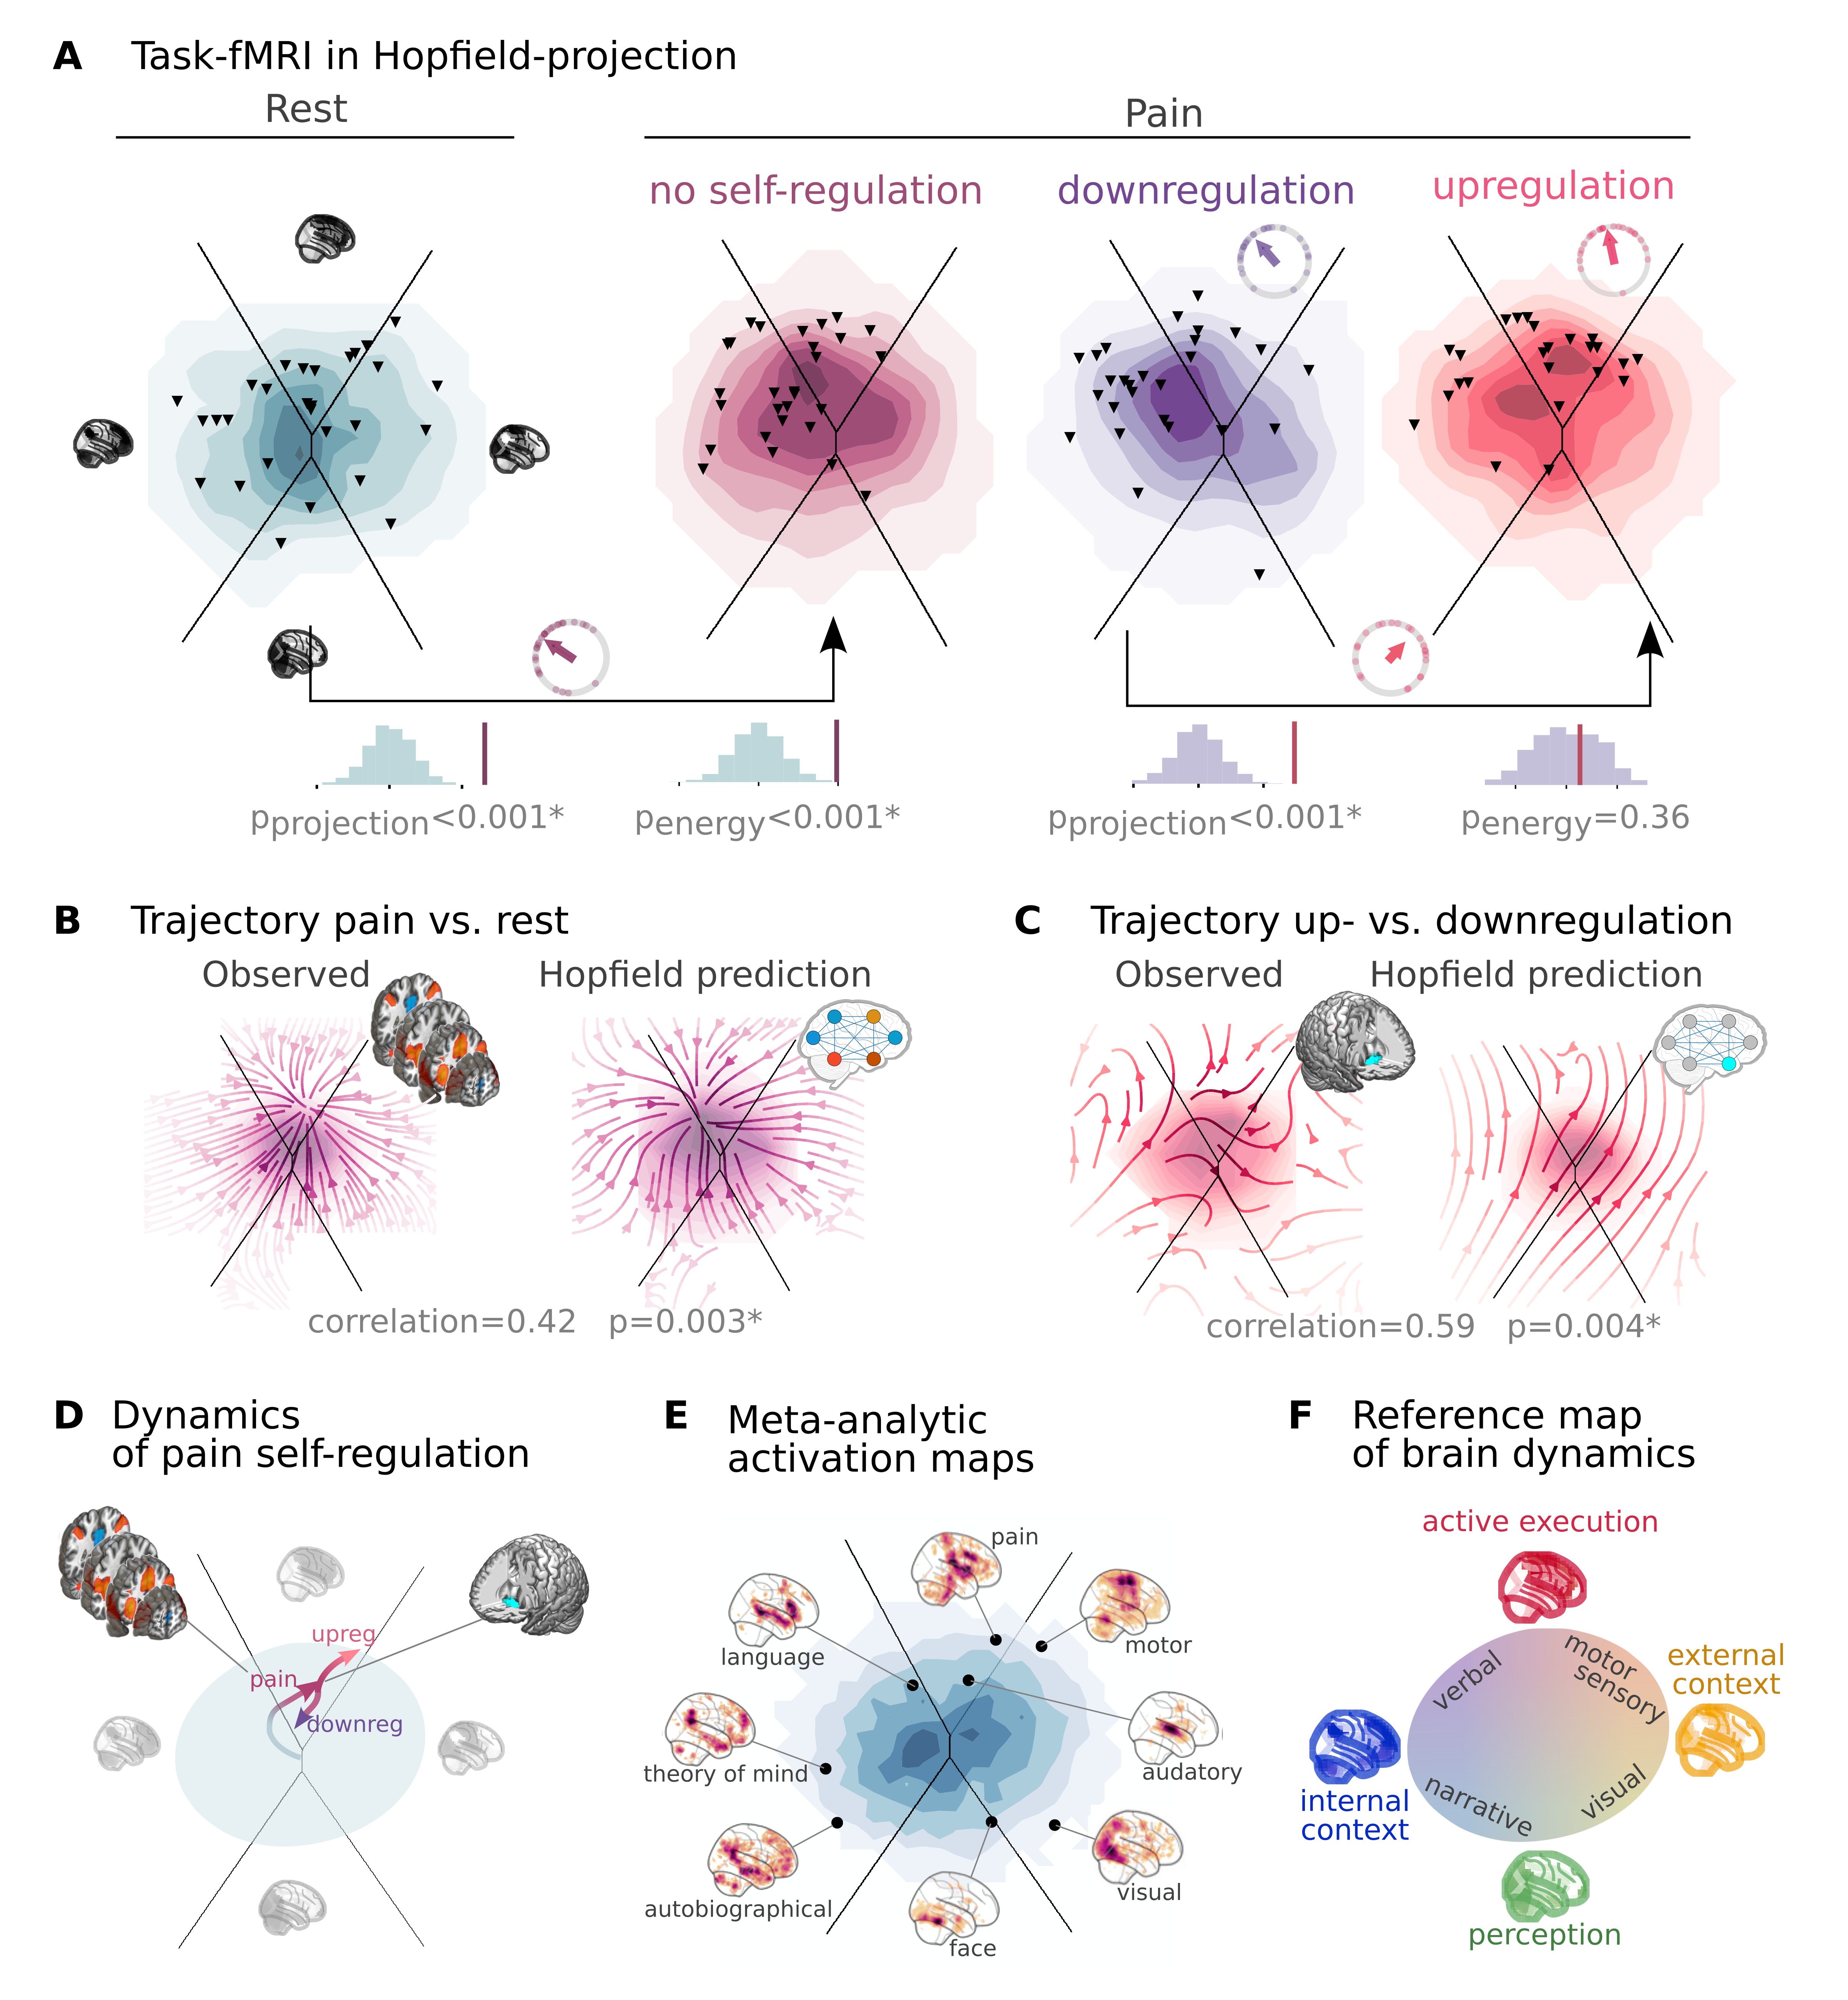
\includegraphics[width=0.7\linewidth]{files/task_validity-50d022af0e838d5db8c143703c965ee6.png}
\caption[]{\textbf{Empirical Hopfield-networks reconstruct real task-based brain activity.} \newline

\textbf{A} Functional MRI time-frames during pain stimulation from Table~\ref{tab-samples} (second Hopfiled projection plot)
and self-regulation (third and fourth) locate significantly differently on the Hopfield projection than brain states
during rest (first projection, permutation test, p\textless 0.001 for all). Energies, as defined by the Hopfield model, are also
significantly different between rest and the pain conditions (permutation test, p\textless 0.001), with higher energies during
pain stimulation. Triangles denote participant-level mean activations in the various blocks (corrected for
hemodynamics). Circle plots show the directions of the change for each individual (points) as well as the mean direction
across participants (arrow), as compared to the reference state (downregulation for the last circle plot, rest for all
other circle plots).
\textbf{B} The average difference between the characteristic directions of the single time-frames on the Hopfield projection
reveal a non-linear flow difference between pain the brain dynamics during pain and rest (left). When introducing weak
pain-related signal in the CBH network during stochastic relaxation, it accurately reproduces these non-linear flow
differences (right).
\textbf{C} Similarly simulating activity in the nucleaus accumbens (NAc) reconstructs a non-linear flow difference between
up- and downregulation (left). When introducing weak self-regulation-related signal similar to the observed dynamics
(characterized by NAc activation differences, as observed by \citep{woo2015distinct}.
\textbf{D} Schematic representation of brain dynamics during pain and its up- and downregulation, visualized on the Hopfield
projection. Pain shifts spontanous brain dynamics towards the "action" subsystem, converging to a putative "ghost
attractor of pain". Up-regulation by NAc de-activation exerts force towards a similar dircetionm while down-regulation
by NAc activation exhibist an opposite effect on brain dynamics, leading to the brain less frequent "visiting"
pain-associated states.
\textbf{E} Visualizing meta-analyitic activation maps on the Hopfiled projection informs our theoretical interpretative
framework
\textbf{F}  for spontaneous and task-based brain dynamics. In the proposed framework, taks-based activity is not a mere
response to external stimuli in certain brain locations but a perturbation of the brain's charcteristic dynamic
trajectories. In this framework, conventional task-based fMRI analyses capture mean differences of the whole brain
dyanmics, resulting in the widely reported focal "activation maps" thought to be specific to various taks and stimuli.
In the CBH framework, the brain's characteristic trajectories are constrained by the underlying functional connectivity
and only perturbed by external inpout, rather than predestinated.}
\label{task-validity}
\end{figure}

These results provide an intuitive account for how the underlying functional connectivity of the brain can give rise to
different activation patterns, depending on the current (extrinsic or intrinsic) input. In the CBH framework, change in
input (i.e. a task or stimulation) does not simply switch to the brain into a distinct "mode" of operation but acts as
a perturbation of the system's dyanmics, resulting in mean activations changes that are only reliable measurable over
an extended period of time, as done by conventional task-based fMRI analyses.

The proposed framework offers much more than visualization and inference of resting state and task based data on the
Hopfield projection. It provides a generative model for observed activity changes, enabling the prediction of brain
activity under different conditions. To illustrate this, we used the CBHs model to simulate brain activity during pain
stimulation and self-regulation. First, we registered the frame-to-frame transitions in the real fMRI data for all four
conditions: rest, pain without self-regulation, downregulation, and upregulation. We then transformed these transitions
into the Hopfield embedding, resulting in two-dimensional vectors on the Hopfield projection for each transition.

Next, we evaluated the average direction in different segments of the projection on a 6x6 grid. Subsequently, we
computed the difference between the mean directions observed during rest and pain (without regulation,
Figure~\ref{task-validity}B, left side), as well as between down- and upregulation (Figure~\ref{task-validity}C, left side).
This analysis unveiled non-linear trajectory patterns, indicating the most probable direction the brain follows from a
specific state (activity pattern) in a particular condition (pain without self-regulation or upregulation), in
comparison to the reference state (rest and downregulation, respectively). In the case of pain versus rest, brain
activity tends to gravitate towards a "ghost attractor" situated near the Hopfield projection of a typical pain
activation map (see e.g. Figure~\ref{task-validity}E). In terms of attractor states, this belongs to the basin of
attractor corresponding to action/execution. In case of up vs. downregulation, brain activity is pulled generally
towards a similar direction, but with a lack of a clear ghost attractor, potentially resulting in more extreme states.

Next, our objective was to evaluate the extent to which the proposed framework can reconstruct these non-linear
dynamics. To simulate the alterations in brain dynamics during pain stimulation, we acquired a meta-analytic pain
activation map \citep{zunhammer2021meta} and incorporated it as an additional signal, along with Gaussian noise,
during the stochastic relaxation procedure. While incorporating such a signal naturally induces a minor linear shift
on the Hopfield projection for each state generated during the stochastic relaxation procedure, this alone could only
marginally explain the observed nonlinear dynamics in the real data (Supplementary material X). After conducting a
coarse-grained optimization across five different signal-to-noise (SNR) values (logarithmically spaced between
0.001 and 0.1), we found that by adding a minimal amount of signal (SNR = 0.01), the CbH model achieved a remarkably
precise reconstruction of the observed non-linear disparities in brain dynamics between the pain and rest conditions,
encompassing the characteristic pain related "ghost attractor". (Spearman's $\rho$ = 0.42, p=0.003,
Figure~\ref{task-validity}B, right side).

The same model was also able to reconstruct the observed non-linear differences in brain dynamics between the up- and
downregulation conditions (Spearman's $\rho$ = 0.59, p=0.004) without any further optimization (SNR=0.01,
Figure~\ref{task-validity}C, right side). The only change we made to the model was the addition (downregulation) or
subtraction (upregulation) of activation in the NAc (the region in which \citep{woo2015distinct} observed significant
changes between up- and downregulation).

These findings offer a novel insight into the neural mechanisms underlying pain and its self-regulation, providing a
mechanistic explanation for the involvement of both nociception-related regions and the NAc (nucleus accumbens) in pain
regulation. (Figure~\ref{task-validity}D). Additionally, these findings emphasize that the conceptual differentiation
between resting and task states may, to a considerable extent, be an artificial dichotomy. Instead, the brain remains
in a continuous state of flux, which is not radically altered by task states, even in the presence of highly salient
stimuli such as pain.

% -> discussion

To provide a comprehensive picture on how other tasks map onto the Hopfield projection, we obtained various task-based
meta-analytic activation maps from Neurosynth (see Supplementary material X for details) and plotted them on the
Hopfield projection (Figure~\ref{task-validity}E). This analysis demonstrated that the Hopfield projection can effectively
visualize and quantify the dynamics of various cognitive processes, encompassing sensory, motor, cognitive, and social
domains. Furthermore, the analysis revealed that the two primary axes of the projection correspond well to the
differentiation between internal and external context, as well as the perception-action axis, respectively.

In this coordinate system, visual processing is labeled "external-perception", sensory-motor processes
"external-active", language, verbal cognition and working memory is labelled "internal-active" and long-term memory
as well as social and autobiographic narrative fall into the "internal-perception" regime (Figure~\ref{task-validity}F).

These results highlight a very powerful feature of the proposed generative framework, namely that it can be used to
simulate and predict brain activity under different conditions. Predicting the effect of lower or higher level of
activity in certain regions, or lower or higher connectivity among them, on global brain dynamics and responses to
various tasks provides unprecedented opportunities for forecasting the effect of interventions, such as pharmacological
or non-invasive brain stimulation, on brain function.

\subsection{Clinical relevance}\label{Clinical relevance}

In our final analysis, we provide a brief outlook towards the potential clinical applications of CBH analysis. We
analyzed three large public clinical databases as provided by the Autism Brain Imaging Data Exchange
(Table~\ref{tab-samples}: ABIDE, \citep{di2014autism}, the Centers of Biomedical Research Excellence
(Table~\ref{tab-samples}: COBRE, \citep{aine2017multimodal}) and the Alzheimer's Disease Neuroimaging Initiative
(Table~\ref{tab-samples}: ADNI, \citep{petersen2010alzheimer}).
Resting state fMRI data of patients with autism spectrum disorder (ASD), schizophrenia (SCZ) and Alzheimer's disease
(AD) was contrasted to their respective control groups (typically developing controls for ASD, healthy control
participants for SCH and individuals with mild cognitive impairment (MCI), respectively). In all three datasets, we used
the CBH model from study 1 and projected the fMRI timeseries of all involved participants onto the Hopfield projection.
For each participant, we obtained the average activation of all time-frames belonging to the same attractor state
(4 maps per participant) and compared these across groups with permutation tests, Bonferroni corrected across brain
regions and attractor states (122*4 comparisons).

We found several significant differences the mean attractor activation of patients as compared to the respective
controls. In ASD, all four attractor activation maps showed significant differences (Figure~\ref{clinical-validity}A,
\textbf{table}), characterized by altered activation in the \textit{precuneus, posterior congulate, sensory-motor system,
posterior insula, and cerebellum}.

In SCZ, the most prominent differences were found in the subsystem for internal context, with elevated activity of
regions that are not typically active in this state, including the \textit{thalamus, the striatum and several cortical regions}
(Figure~\ref{clinical-validity}B, \textbf{table}). Additional activation increases in \textit{visual and motor} areas were observed in
the active inference subsystem.

In the AD vs. MCI comparison, we found significant differences in two of the four attractor activation maps
(Figure~\ref{clinical-validity}C, \textbf{table}), indicating changes in the resting state activity of subsystems for passive
inference and internal context (both of which together host long-term memory processes, see Figure~\ref{task-validity}F).
At the regional level, differences are characterized by altered activation in the \textit{dorsolateral prefrontal cortex
(DLPFC) and the cerebellum}.

\begin{figure}[!htbp]
\centering

\includegraphics[width=0.7\linewidth]{files/state_analysis-6a1e0e3c85e7f52218ce946cff5ad7d2.svg}
\caption[]{\textbf{Connectome-based Hopfield analysis as a sensitive tool for the study of clinical disorders.} \newline
\textless {\textbackslash}br\textgreater 
We quantified attractor state activations in three clincal datasets ((Table~\ref{tab-samples}) as the
individual-level mean activation of all time-frames belonging to the same attractor state. CBH analysis of attractor
state activations revealed significant differences in all three datasets.
\textbf{A} Comparison of individuals with autism spectrum disorder (ASD) and typically developing controls (TD) is
characterized by \textbf{todo}.
\textbf{B} The most prominent Schizophrenia (SCZ)-related differences (as compared to healthy controls (HC) are related to
the activity of the internalalization-related subsystem. \textbf{todo}
\textbf{C} Alzheimer's disease (AD) is characterized by altered activation in \textbf{todo} the subsystems for passive inference
and internal context (both of which together host long-term memory processes, see Figure~\ref{task-validity}F). All
results are corrected for multiple comparisons across brain regions and attractor states (122*4 comparisons)
with Bonferroni-correction. See Table \textbf{X} for detailed results.}
\label{clinical-validity}
\end{figure}

\section{Discussion}\label{Discussion}

Regions of the brain engage in an ongoing exchange of information, leading to co-activations that are commonly known as
functional connectivity. The quantity of information exchanged between brain regions is not uniform, but rather exhibits
substantial variation among different pairs of regions, encompassing the intricate network referred to as the functional
connectome. In this study, we have introduced a simple yet robust model that elucidates how activity propagates through
the intricate network topology of the brain, thereby constraining the system's dynamics and giving rise to distinct
brain states along with characteristic dynamic responses to perturbations. Through a series of experiments, we have
demonstrated that the proposed model can effectively reconstruct and predict large-scale brain activity across diverse
conditions. These findings offer unprecedented possibilities for forecasting the impact of interventions, including
pharmacological treatments or non-invasive brain stimulation, on brain function.

The construct validity of our model is rooted in the activity flow principle, first introduced by
\citep{cole2016activity}. The activity flow principle states that functional connectivity between regions A and B can
be conceptualized as the degree to which activity is transferred form A to B. This principle has been shown to
successfully predict held out brain activations by a weighted sum of the activations of all the regions where the
weights are set to the functional connectivity of those regions to the held-out region
\citep{cole2016activity, ito2017cognitive, mill2022network, hearne2021activity, chen2018human}.

\begin{quote}
ToDo: latent FC-based modelling: \cite{McCormick_2022}
\end{quote}

Our model was born from the intuition that the repeated, iterative application of the activity flow equation results in
a system showing close analogies with a type of recurrent artificial neural network, know as Hopfield networks
\citep{hopfield1982neural}.

Hopfield networks have previously been shown to exhibit a series of characteristics that are also highly relevant for
brain function, including the ability to store and recall memories \citep{hopfield1982neural}, self-repair (\textbf{ref}),
a staggering robustness to noisy or corrupted inputs \citep{hertz1991introduction} and the tendency to produce
multistable dynamics organized by the "gravitational pull" of a finite number of attractor states
\citep{khona2022attractor}.

The proposed link between activity flow and Hopfield networks has an important implication: network weights must be
initialized with functional connectivity values, (specifically, partial correlations, as recommend by
\citep{cole2016activity}, instead of applying an explicit training procedure (common in the "neuroconnectomist"
approach \citep{doerig2023neuroconnectionist}) or using the structural connectome (a standard practice of conventional
computational neuroscience \citep{cabral2017functional}.

Using functional conncetome-based Hopfield (CBH) model provides a simple yet powerful framework for the mechanistic
understanding of brian dynamics. Its simplicity comes with important advantages.

First, increasing model complexity results in an exponential explosion of the parameter space. Although complex,
fine-grained computation models hold promise a full-blown understanding, they very easily overfit real data (\textbf{ref}).
The basic CBH approach has only two hyperparameters (temperature and noise) and produce fairly consistent behavior on a
wide range of parameter values. To demonstrate the power of simplicity, in the present work, we deliberately minimized
fine-tuning of any free parameters. We fixed the temperature parameter at a value that robustly provides 4 attractor
states and used a single noise level for all experiments (selected with a coarse optimization procedure to approximately
mimic the distribution of real data).

Second, increasing complexity means increasing burden in terms of interpretability. The CBH model establishes a simple
and direct link between two most popular measures of brain function: functional connectivity and brain activity. This
link is not only conceptual, but also mathematical, and allows us to investigate and forecast changes of the system's
dyanmics in response to perturbations of both activity and connectivity.

In this initial investigation, we further reduced complexity by restricting the analysis to a simplified 2-dimensional
embedding of the state-space generated by the CBH approach, which we refer to as the Hopfield projection. This
projection is a powerful tool for the visualization of the CBH model's dynamics, and allows for a direct comparison
with the dynamics of the original brain activity.

However, the Hopfield projection only conveys a small proportion of the richness of the full state-space dynamics
reconstructed by the CBH model. Investigating higher-dimensional dynamics, fine-tuned hyperparameters, the effect of
different initializations and perturbations is an important direction for future work, with the potential to further
improve the model's accuracy and usefulness.

Given these intentional simplifications, it is remarkable, if not surprising, how accurately the CBH model is able to
reconstruct and predict brain dynamics under a wide range of conditions. Next to accurately reconstructing the
distribution of, and the time spent in, different brain states during resting state, its superiority in explaining, and
generalizing to, resting state brain activation patterns over principal components derived from the same data is
particularly striking. The question arises, how can a relatively simple model, which is informed about empirical brain
dynamics only through the functional connectome, be so powerful? A possible answer is that, while empirical data (and
its principal components) are corrupted by noise and low sampling rate, the highly noise tolerant nature and the
self-repair properties of the CBH architecture allow it to capture and reconstruct the basic principles of the
underlying dynamics.

The noise-tolerance of the proposed architecture also explains the high replicability of CBH attractors across different
datasets (study 2 and 3). The observed level of replicability allowed us to re-use the CBH model constructed with the
connectome of study 1 for all subsequent studies, without any further fine-tuning or study-specific parameter
optimization.

The connectome obtained form study 1 was also used to evaluate the model's ability to capture and forecast task-induced
brain dynamics in study 4 and 5. In these analyses, the CBH model was not only able to capture participant-level
activity changes induced by pain and self-regulation (showing significant differences on the Hopfield projection and in
terms of state energy), but also accurately predicted the non-linear changes in activity flow induced by characteristic
activity changes.

Brain dynamics can not only be perturbed by task or other types of experimental or naturalistic interventions, but also
by pathological alterations. In our analysis of clinical samples study 6-8 we found that mean attractor activations show
characteristic alteration in autism spectrum disorder (ASD), Schizophrenia (SCH) and Alzheimer's disease (AD). These
changes were also detectable on the Hopfield projection, and were accompanied by significant changes in the state
energies. The Hopfiled projection also allowed us to visualize the effect of different types of perturbations on the
brain's attractor landscape, providing a novel perspective on the pathophysiology of these disorders.

\begin{quote}
ToDo: more details on clinical outlook
\end{quote}

\begin{quote}
ToDo: discuss: what are attractor states at all? Platonic idealizations of brain states, that are continously approximated by the brain?
\end{quote}

\begin{quote}
Todo: for spontaneous and task-based brain dynamics. In the proposed framework, taks-based activity is not a mere response to external stimuli in certain brain locations but a perturbation of the brain's charcteristic dynamic trajectories. In this framework, conventional task-based fMRI analyses capture mean differences of the whole brain dyanmics, resulting in the widely reported focal "activation maps" thought to be specific to various taks and stimuli. In the CBH framework, the brain's characteristic trajectories are constrained by the underlying functional connectivity and only perturbed by external inpout, rather than predestinated.
\end{quote}

\begin{quote}
ToDo: discuss: the CBH model is not a model of brain function, but a model of brain dynamics. It does not strice to explain various brain regions ability to perform certain computations, but the brain's characteristic trajectories, which are perturbed by tasks and other types of interventions.
\end{quote}

Together, these results open up a series of exciting opportunities for the mechanistic understanding of brain function.
By its generative nature, the CBH model could foster analyses that aim at disentangling causal relationships, which are
extremely difficult to infer in case of systems as complex as the brain. It could, for instance, aid the differentiation
of primary causes and secondary effects of particular activity or connectivity changes in various clinical conditions.

Moreover, the CBH approach might provide testable predictions about the effects of interventions on brain functions,
like pharmacological or non-invasive brain stimulation (e.g. transcranial magnetic or direct current stimulation,
focused ultrasound) or neurofeedback.
For instance, in the context of pain, the CBH model might be used to predict the effect of various analgesic drugs (or
other treatment strategies with known neural correlates) on the individual level (e.g. based on the individual
functional connectome). Aiding the design of personalized medicine approaches is a particularly promising field of
application for the proposed framework.

The generative nature of the proposed framework may be also used to generate synthetic brain activity data, which can
be used to train and test machine learning algorithms, such as deep neural networks, for the prediction of brain
activity from functional connectivity. This approach may be particularly useful in the context of clinical applications,
where the amount of available data is often limited.

\section{Conclusion}\label{Conclusion}

To conclude, here we have proposed a novel computational framework that accurately captures and predicts brain dynamics
under a wide range of conditions. The framework models large-scale activity flow in the brain with a recurrent
artificial neural network architecture that, instead of being trained to solve specific tasks or mimic certain dynamics,
is simply initialized with the empirical functional connectome. The framework identifies biologically meaningful
attractor states and provides a model for how these restrict brain dynamics. The proposed framework, referred to as the
connectome-based Hopfield (CBH) model, can accurately reconstruct and predict brain dynamics under a wide range of
conditions, including resting state, task-induced activity changes, and pathological alterations. CBH analyses provide
a simple, robust, and highly interpretable computational alternative to the conventional descriptive approach to
investigating brain function and establish a link between connectivity and activity. The generative nature of the
proposed model opens up a series of exciting opportunities for future research, including novel ways of assessing
causality and mechanistic understanding, and the possibility to predict the effects of various interventions, thereby
paving the way for novel personalized medical approaches.

\section{Methods}\label{Methods}

\begin{table}
\centering
\begin{tabular}{p{\dimexpr 0.143\linewidth-2\tabcolsep}p{\dimexpr 0.143\linewidth-2\tabcolsep}p{\dimexpr 0.143\linewidth-2\tabcolsep}p{\dimexpr 0.143\linewidth-2\tabcolsep}p{\dimexpr 0.143\linewidth-2\tabcolsep}p{\dimexpr 0.143\linewidth-2\tabcolsep}p{\dimexpr 0.143\linewidth-2\tabcolsep}}
\toprule
study & modality & analysis & n & age (mean$\pm$sd) & \%female & references \\
\hline
study 1 & resting state & discovery & 41 & 26.1$\pm$3.9 & 37\% & \cite{Spisak_2020} \\
study 2 & resting state & replication & 48 & 24.9$\pm$3.5 & 54\% & \cite{Spisak_2020} \\
study 3 & resting state & replication & 29 & 24.8$\pm$3.1 & 53\% & \cite{Spisak_2020} \\
study 4 & task-based & pain self-regulation & 33 & 27.9 $\pm$ 9.0 & 66\% & \cite{Woo_2015} \\
study 5 (Neurosynth) & task-based & coordinate-based meta-analyses & 14371 studies in total & \textbullet~~\newline
 & \textbullet~~\newline
 & \cite{Tor_D__2011} \\
study 6 (ABIDE, NYU sample) & resting state & Autism Spectrum Disorder & ASD: 98, NC: 74 & 15.3$\pm$6.6 & 20.9\% & \citep{di2014autism} \\
study 7 (ADNI) & resting state & Alzheimer's Disease vs. Mild Cognitive Impairment & AD: 34, MCI 99: & 72.5$\pm$7.5 & 50.4\% & \citep{petersen2010alzheimer} \\
study 8 (COBRE) & resting state & Schizophrenia & SCH: 60, HC: 72 & 37.0$\pm$12.6 & 29.4 \% & \citep{aine2017multimodal} \\
\bottomrule
\end{tabular}
\end{table}

\subsection{Hopfield network}\label{Hopfield network}

The weights $w_{ij}$ have to be symmetric and the diagonal elements are set to zero.

Todo

Todo



\bibliographystyle{unsrtnat}
\bibliography{main.bib}

\end{document}
